\section{Experiments}

From a series of simulated electron showers our conditional GAN is tasked with learning the simulated data distributions generated by \geant. There exist several methods to estimate the performance of generative models, but not all evaluation criteria are equally suitable and reliable for all applications. In our paper we focus on quantitative evaluation based on physics-driven similarity metrics. The choice reflects the domain specific procedure for data-simulation comparison. 

Examples of real and produced images are presented in~\cref{fig:gen-imgs-2}. It can be concluded that produced images look quite similar to the original data but we are also supposed to do more deep analysis.

\begin{figure}
\captionsetup[subfigure]{justification=centering}
  \centering
  \begin{subfigure}{0.24\textwidth}
    \centering
    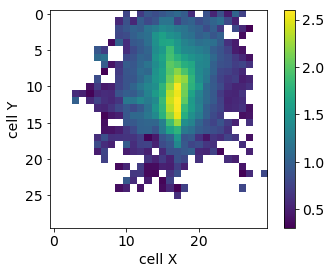
\includegraphics[width=1\textwidth]{figures/1_real.png}
    \caption{\\$E = 63.7~\text{GeV}$ \\ $\frac{p_x}{p_z}=0.005$ \\ $\frac{p_y}{p_z}=0.154$}\label{fig:real-imgs-1}
  \end{subfigure}
  \begin{subfigure}{0.24\textwidth}
    \centering
    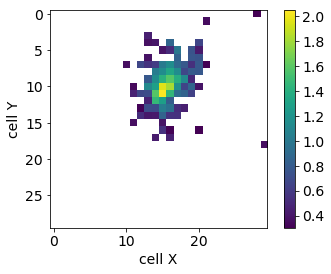
\includegraphics[width=1\textwidth]{figures/2_real.png}
    \caption{\\$E = 6.5~\text{GeV}$ \\  $\frac{p_x}{p_z}=0.0046$ \\$\frac{p_y}{p_z}=0.108$}\label{fig:real-imgs-2}
  \end{subfigure}
    \begin{subfigure}{0.24\textwidth}
    \centering
    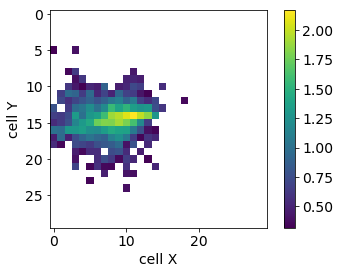
\includegraphics[width=1\textwidth]{figures/3_real.png}
    \caption{\\$E = 15.6~\text{GeV}$ \\ $\frac{p_x}{p_z}=0.196$ \\ $\frac{p_y}{p_z}=-0.036$}\label{fig:real-imgs-3}
  \end{subfigure}
  \begin{subfigure}{0.24\textwidth}
    \centering
    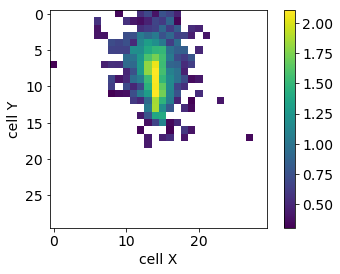
\includegraphics[width=1\textwidth]{figures/4_real.png}
    \caption{\\$E = 15.6~\text{GeV}$ \\  $\frac{p_x}{p_z}=-0.019$ \\ $\frac{p_y}{p_z}=0.181$}\label{fig:real-imgs-4}
  \end{subfigure}
  \caption{Images and the parameters from the real dataset. \todo{generate high quality images}}
  \label{fig:real-imgs}
\end{figure}


\begin{figure}
\captionsetup[subfigure]{justification=centering}
  \centering
  \begin{subfigure}{0.24\textwidth}
    \centering
    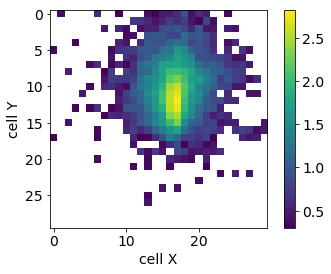
\includegraphics[width=1\textwidth]{figures/1_gen.png}
    \caption{\\$E = 63.7~\text{GeV}$ \\ $\frac{p_x}{p_z}=0.005$ \\ $\frac{p_y}{p_z}=0.154$}\label{fig:gen-imgs-1}
  \end{subfigure}
  \begin{subfigure}{0.24\textwidth}
    \centering
    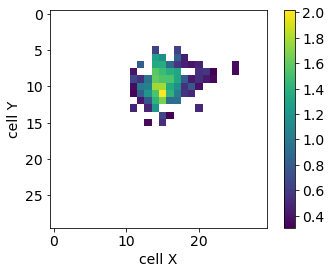
\includegraphics[width=1\textwidth]{figures/2_gen.png}
    \caption{\\$E = 6.5~\text{GeV}$ \\  $\frac{p_x}{p_z}=0.0046$ \\$\frac{p_y}{p_z}=0.108$}\label{fig:gen-imgs-2}
  \end{subfigure}
    \begin{subfigure}{0.24\textwidth}
    \centering
    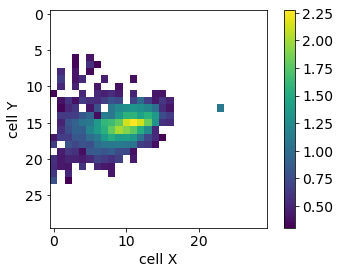
\includegraphics[width=1\textwidth]{figures/3_gen.png}
    \caption{\\$E = 15.6~\text{GeV}$ \\ $\frac{p_x}{p_z}=0.196$ \\ $\frac{p_y}{p_z}=-0.036$}\label{fig:gen-imgs-3}
  \end{subfigure}
  \begin{subfigure}{0.24\textwidth}
    \centering
    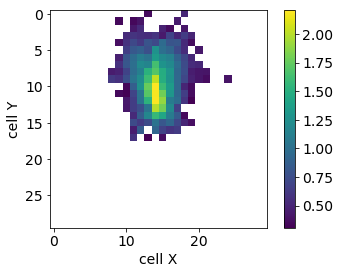
\includegraphics[width=1\textwidth]{figures/4_gen.png}
    \caption{\\$E = 15.6~\text{GeV}$ \\  $\frac{p_x}{p_z}=-0.019$ \\ $\frac{p_y}{p_z}=0.181$}\label{fig:gen-imgs-4}
  \end{subfigure}
  \caption{Images and the parameters from the real dataset. \todo{generate high quality images}}
  \label{fig:gen-imgs}
\end{figure}


As a part of the analyzing generated images quality we calculated some physical characteristics of shower shapes such as cluster asymmetry, shower width and sparsity level. The obtained characteristics are presented in~\cref{fig:quality}. How to calculate these variables is described in Appendix.

\begin{figure}
  \centering
  \centering
  \begin{subfigure}{0.19\textwidth}
    \centering
    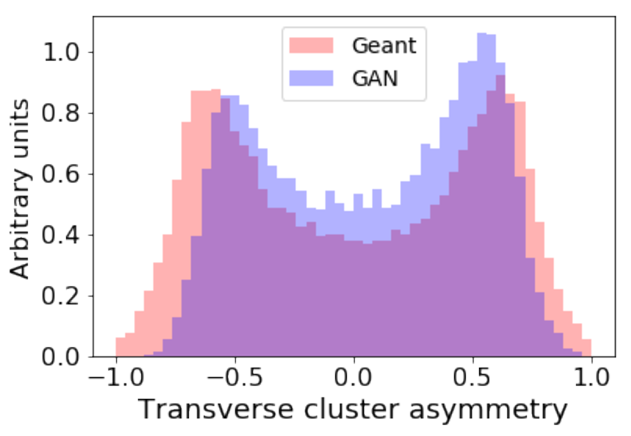
\includegraphics[width=1\textwidth]{figures/transverseAsymmetry.pdf}
    \caption{The transverse asymmetry of real and generated images}
  \end{subfigure}
  \begin{subfigure}{0.19\textwidth}
    \centering
    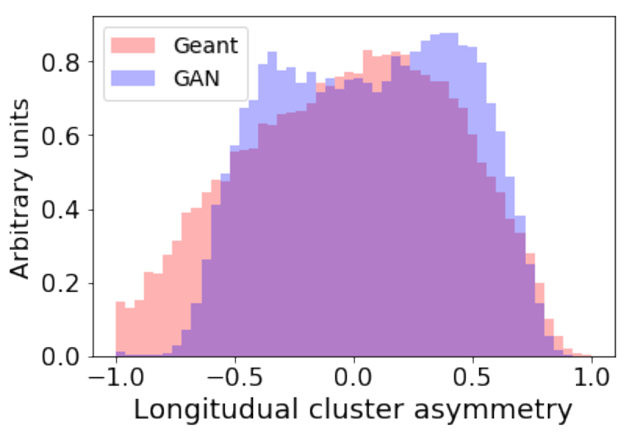
\includegraphics[width=1\textwidth]{figures/longAsymmetry.pdf}
    \caption{The longitudal asymmetry of real and generated images}
  \end{subfigure}
  \begin{subfigure}{0.19\textwidth}
    \centering
    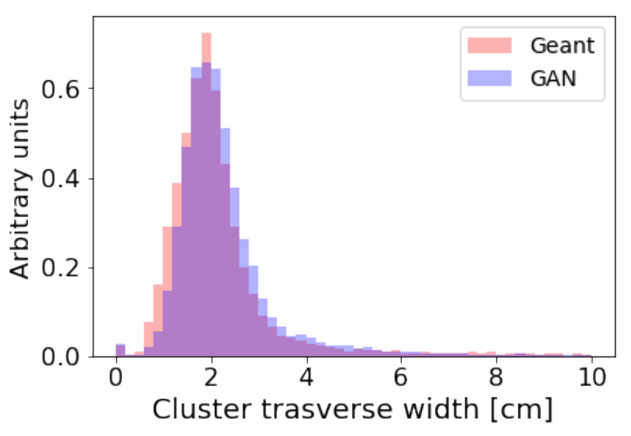
\includegraphics[width=1\textwidth]{figures/width.pdf}
    \caption{The transverse width of real and generated images}
  \end{subfigure}
  \begin{subfigure}{0.19\textwidth}
    \centering
    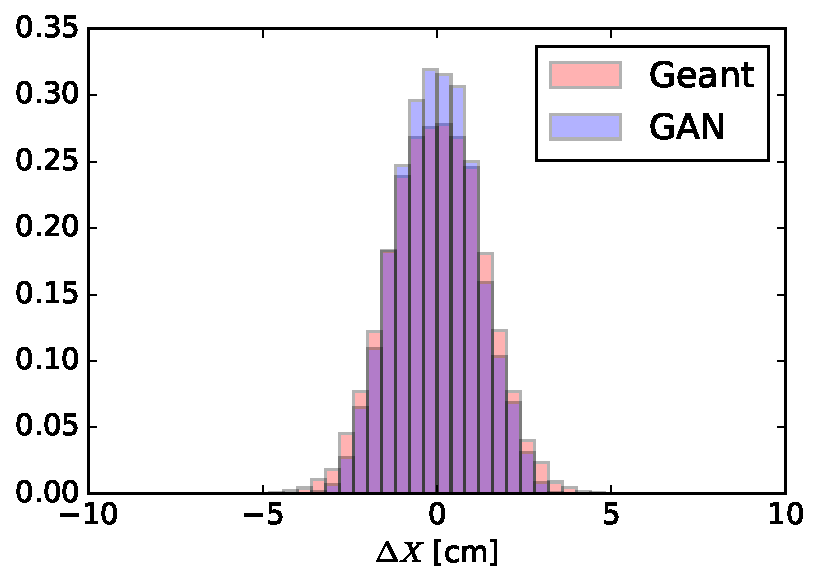
\includegraphics[width=1\textwidth]{figures/deltaX.pdf}
    \caption{Delta X}
  \end{subfigure}
  \begin{subfigure}{0.19\textwidth}
    \centering
    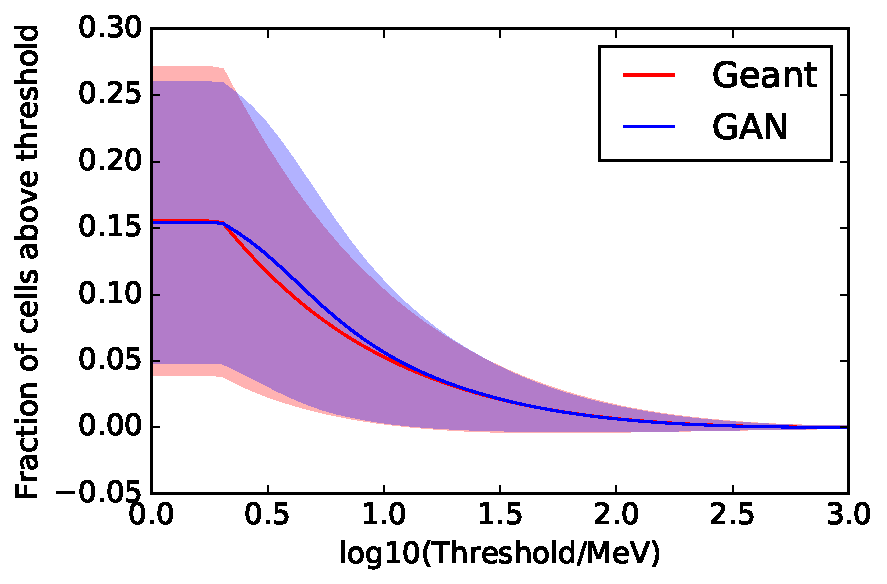
\includegraphics[width=1\textwidth]{figures/sparsity.pdf}
    \caption{The sparsity of real and generated images}
  \end{subfigure}
  \caption{Generated images quality evaluation including described physical characteristics.}\label{fig:quality}  
\end{figure}

The results are in good agreement with fully simulated data. Energy showers are faithfully reproduced and show a reasonable agreement with the standard Monte Carlo techniques. A detailed study to asses the quality of the GAN images using typical high level calorimeter reconstruction variables confirms this statement.

As for model performance, we trained our model for 3000 epochs which takes about 70 hours on GPU NVIDIA Tesla K80. The sampling rate is 0.07 ms per sample on GPU, 4.9 ms per sample on CPU.
